\chapter{可预测预训练技术应用--MiniCPM-2B}

\section{基于WSD调度器的多阶段训练策略}
\label{sec:trainingstrategy}
通常,遵循指令的大语言模型(LLMs)的训练包含预训练阶段和监督微调(SFT)阶段~\citep{zhang2023instruction,wei2021finetuned}。在预训练阶段,数据由大规模无标签数据组成,而在监督微调阶段,高质量的有标签数据成为优化目标。

鉴于在WSD学习率调度器的衰减阶段观察到的显著损失下降,我们假设在此阶段整合高质量的有标签数据具有双重优势:
\begin{itemize}
    \item 除了在监督微调阶段,在退火阶段引入此类数据有助于模型进行更全面的学习。具体而言,相较于预训练数据分布,它能促使模型在针对监督微调数据分布时实现更显著的损失降低。这种方式与实际用户场景更为契合。
    \item 与在整个预训练过程中均匀分布高质量数据不同,此方法通过集中处理数据并维持持续预训练来提升训练效果。如果我们不预先确定训练步数,在持续的预训练过程中重复使用小数据集可能会产生负面影响。
\end{itemize}

基于这两个假设,我们提出以下训练策略:在预训练阶段,仅使用大规模的粗质量预训练数据,这类数据丰富,且在提供更多计算资源时能够支持持续训练。在退火阶段,我们使用多样且高质量的、面向知识与能力的监督微调数据,并将其混入预训练数据中。

为验证我们训练策略的优势,我们使用(A) MiniCPM - 2.4B稳定阶段的中间检查点和(B) MiniCPM - 1.2B稳定阶段的最后检查点进行对比实验。具体来说,我们比较以下几种情况:

\begin{enumerate}
    \item A - 1:24亿参数模型,仅使用预训练数据进行衰减,随后进行40亿词元的监督微调。
    \item A - 2:24亿参数模型,使用上述混入预训练数据中的高质量无标签数据和监督微调数据进行衰减,随后也进行40亿词元的监督微调。
    \item B - 1:12亿参数模型,仅使用预训练数据进行衰减,随后进行60亿词元的监督微调。
    \item B - 2:12亿参数模型,仅使用预训练数据进行衰减,随后进行120亿词元的监督微调。
    \item B - 3:12亿参数模型,使用上述混入预训练数据中的高质量数据 + 监督微调数据进行退火,随后也进行60亿词元的监督微调。 
\end{enumerate}

实验结果如表\ref{tab:dataexperiments}所示。我们可以看到,尽管A - 2和A - 1经历了相同的监督微调数据分布,但在衰减阶段添加监督微调数据提升了模型表现。B - 2和B - 3的比较表明,仅进行监督微调的不足并非源于监督微调阶段训练词元不足。 

\begin{table}[h]
\centering
\begin{tabular}{lccccccc}
\toprule
            & \textbf{C - Eval} & \textbf{CMMLU} & \textbf{MMLU} & \textbf{GSM8K} & \textbf{MATH} & \textbf{HumanEval} & \textbf{MBPP} \\ \midrule
A - 1 & 40.0  & 41.5  & 44.6 & 27.7  & 5.1  & 27.7      & 24.4 \\
A - 2 & \textbf{52.6}  & \textbf{51.1} & \textbf{50.9} & \textbf{42.3 } & \textbf{5.4}  & \textbf{30.4 }     & \textbf{30.3} \\
\midrule

B - 1 &   40.9  & 41.5 & 47.9 &  34.2 & 7.9   &  43.9 & 30.5 \\
B - 2 &  41.2 &  42.0 &    47.9  & \textbf{34.4} & 7.3 &  43.9 & 29.8  \\ 
B - 3 & \textbf{49.1}  & \textbf{46.8}  & \textbf{49.6} & 31.8  & \textbf{10.5}  & \textbf{44.5}  & \textbf{32.8}\\
% B - 4 & 43.9 & 45.3 &  50.1 & 39.3 & 10.1 & 45.1 & 33.5 \\
\bottomrule
\end{tabular}
\caption{不同训练策略的消融研究。
}
\label{tab:dataexperiments}
\end{table}

结果表明,在衰减阶段开始时引入高质量数据的益处远高于仅在监督微调阶段添加。因此,我们建议模型能力的专业化和增强应从衰减阶段开始。 

\section{MiniCPM系列}


在本节中,我们将介绍MiniCPM,这是一系列小语言模型,主要基于两个模型构建,分别具有24亿和12亿非嵌入参数,在各自的20亿和10亿规模类别中表现卓越。MiniCPM还展现出与70亿 - 130亿参数规模的语言模型相当的能力,如Llama2 - 7B~\citep{touvron2023llama}、Mistral - 7B~\citep{jiang2023mistral}、Gemma - 7B~\citep{Banks2024Gemma}以及Llama - 13B~\citep{touvron2023llama}等。尽管模型规模较小,但我们精心设计了训练方法,以便在模型规模和数据范围上实现无缝扩展。这在我们的模型风洞实验中得到了体现,其中包括全面的超参数优化(第\ref{MWTE}节),以及采用WSD(预热 - 稳定 - 衰减)学习率调度器(第\ref{sec:wsdlrs}节)。后者专为在预训练token数量未预先定义的情况下进行连续训练而设计,使得模型中间检查点的重用极具可行性。我们对MiniCPM的训练动态进行了详细分析,结果表明WSD调度器展现了模型预训练中有趣的损失景观。借助WSD调度器,我们现在还能够以在模型轴上的线性工作量和在数据轴上的可忽略工作量来研究数据 - 模型缩放定律,而传统方法在考虑模型和数据轴的缩放时需要二次工作量。缩放定律的结果表明,与Chinchilla最优缩放相比,其数据大小与模型大小的比率要高得多~\citep{hoffmann2022training}。

此外,我们还介绍了MiniCPM家族,包括MiniCPM - DPO、MiniCPM - 128K和MiniCPM - MoE。我们针对既定基准对MiniCPM家族进行了评估,彰显了它们作为小语言模型令人瞩目的能力:(1)基础模型超越了Mistral - 7B和LLama - 13B。(2)DPO模型在MTBench~\citep{zheng2024judging}上超越了zephyr - 7B~\citep{tunstall2023zephyr}。(3)24亿参数的MiniCPM - 128K模型的性能超越或与Yarn - Mistral - 7B - 128K~\citep{peng2023yarn}和ChatGLM3 - 6B - 128K~\citep{du2021glm}等模型相当。(4)具有40亿激活参数的MiniCPM - MoE与Llama2 - 34B~\citep{touvron2023llama}不相上下。

总之,MiniCPM开启了小语言模型发展的新阶段,例证了小语言模型的潜在能力,并倡导以更科学、可持续的方式扩大大语言模型的规模。 



\section{模型基本配置}
在本节中,我们开始介绍融合了上述观察结果与技术的MiniCPM模型。
\label{sec:model}
\begin{table}[htbp]
    \centering
\scalebox{0.90}{
    \begin{tabular}{l|ccccccccc}
    \toprule
        模型 & N(十亿)& $d_m$ & $d_{ff}$ & $d_h$ & $n_q$ & $n_{kv}$ & $L$ & 批量大小(百万) & 词元数(T)\\
    \midrule
       MiniCPM - 1.2B & 1,247,442,432  & 1,536 & 3,840 & 64 & 24 & 8 & 52 & 200万 $\rightarrow$ 400万 & 1.1T\\
       MiniCPM - 2.4B & 2,442,057,984 & 2,304 & 5,760 & 64 & 36 & 36 & 40 & 400万 &  1.1T\\
    \bottomrule
    \end{tabular}
}
    \caption{MiniCPM的模型配置。N(十亿)、$d_m$、$d_{ff}$、$d_h$、$n_q$、$n_{kv}$、$L$、批量大小(百万)、词元数(T)分别代表模型的非嵌入参数数量、模型隐藏维度、前馈层瓶颈维度、注意力头维度、查询数量、键/值数量、层数、训练批量大小、总训练词元数。}
    \label{tab:model_configs}
\end{table}

\section{词表}
尽管MiniCPM的参数规模较小,但其目标是对多样的数据分布进行建模,在中英文方面表现出色。因此,我们的词表相对较大。对于24亿参数的模型,我们使用了由122,753个词元组成的分词器(记为MiniCPMTokenizer - 120K)。这个词表是从广泛多样的语言数据中构建而成,利用sentencepiece库\footnote{\url{https://github.com/google/sentencepiece}}进行字节对编码(BPE)~\citep{sennrich-etal-2016-neural},并且包含了诸如繁体字、生僻字、表情符号以及希腊字母、西里尔字母等特殊符号。

对于小语言模型(SLM)而言,如果词表较大,嵌入参数会占用大量的参数空间。因此,对于我们12亿参数的模型,我们使用了一个更小的词表MiniCPMTokenizer - 70K。与MiniCPMTokenizer - 120K分词器相比,我们在相同文档上重新训练了分词,同时将最大词表数量设置为64,000。对于特殊字符,我们仅添加了繁体字、表情符号和特殊符号,但省略了中文生僻字。

我们对未包含在分词器训练集中的30万篇中文、英文、代码和学术论文文档进行了评估。MiniCPM - 120K分词器实现了最高的压缩率(字节/词元)。

\begin{table}[htbp]
    \centering
    \begin{tabular}{lccccc}
    \toprule
      & {\textbf{百川2}}  & {\textbf{ChatGLM2}} & {\textbf{Llama2}} & {\textbf{MiniCPM - 120K}}  & {\textbf{MiniCPM - 70K}}\\
    \midrule
    词表大小 & 125,696 & 64,794 & 32,000 & 122,753 & 73,440\\
    \midrule
    \multicolumn{6}{c}{\textbf{压缩率}(字节/词元) }\\
    \midrule
    中文 & 3.64   & 3.54  & 1.87  & \textbf{3.73} &  3.56 \\
    英文 & 4.12   & 4.02  & 3.78  & \textbf{4.14} & 4.02 \\
    代码    & 2.71   & 2.71  & 2.74  & \textbf{2.81} & 2.76 \\
    论文   & 2.74   & 2.88  & \textbf{2.97}  & 2.93 & 2.88\\
    \midrule
    平均 & 3.30   & 3.29  & 2.84  & \textbf{3.40}  & 3.31 \\
    \bottomrule
    \end{tabular}
    \caption{压缩率对比。}
    \label{tab:compression_ratio}
\end{table}
    

\section{模型细节}
\subsubsection{模型细节}
\noindent\textbf{词表}:对于MiniCPM - 2.4B,我们使用词表大小为122,753的分词器;对于MiniCPM - 1.2B,使用词表大小为73,440的分词器。12亿参数模型采用较小词表有助于提升效率,且不会过多损害性能。分词器的详细信息见附录\ref{app:tokenizer}。包含嵌入参数后,总参数分别增加了3亿和2亿。 

\noindent\textbf{共享输入 - 输出层}:对于小语言模型(SLM),嵌入会占用较大的参数空间。为减小模型参数规模,MiniCPM - 2.4B和MiniCPM - 1.2B都采用了嵌入共享技术。 
% 对于24亿参数模型,得到的嵌入参数为$2304 \times 122753 = 0.28B$;对于12亿参数模型,约为$1536 \times  \sim 0.11B$。 

\noindent\textbf{深而窄的网络}:在训练MiniCPM - 1.2B之前,我们先训练了MiniCPM - 2.4B。与Phi - 2~\citep{Javaheripi2023Phi2}相比,训练MiniCPM - 2.4B时,我们采用了更深且更窄的架构(40层,而Phi - 2为32层)。最近,~\cite{liu2024mobilellm}提出为小语言模型训练深而窄的网络,这与我们的观点一致。因此,对于MiniCPM - 1.2B,我们进一步加深并收窄了其架构。 

\noindent\textbf{组查询注意力}:我们在训练MiniCPM - 2.4B时,对注意力层未做修改。而受~\cite{liu2024mobilellm}启发,我们在MiniCPM - 1.2B中应用了组查询注意力(Group Query Attention)~\citep{ainslie-etal-2023-gqa},以进一步减少参数数量。

\section{训练阶段}
MiniCPM基础模型的整体训练包括三个阶段:稳定训练阶段、衰减阶段、监督微调(SFT)阶段~\citep{zhang2023instruction,wei2021finetuned}。在整个训练过程中,我们使用Adam优化器~\citep{kingma2014adam}。 

\textbf{稳定训练阶段}:我们使用了约1万亿的数据(数据分布见\ref{fig:appdatamixture}节),其中大部分数据来自公开数据集。我们采用在模型风洞实验中发现的最优配置,即WSD学习率调度器(WSD LRS),批量大小为393万,最大学习率为0.01。

\textbf{衰减阶段}:我们使用预训练数据和高质量监督微调(SFT)数据的混合数据。
对于WSD调度器的具体退火形式,我们采用指数退火,即$f(s - T)=  0.5^{(s - S)/T}$,其中$T$设置为5000步(200亿词元)。

\textbf{监督微调(SFT)阶段}:我们发现仍然有必要进行单独的监督微调阶段。我们使用与退火阶段类似的监督微调数据,但不包含预训练数据,并使用约60亿词元进行训练。监督微调的学习率与退火结束时的学习率一致,并且也采用带有指数衰减的WSD调度器。 





\section{训练数据分布}
\label{sec:appdatadistrbution}

\begin{figure}[htbp]
    \centering
    \begin{minipage}{0.48\linewidth}
        \centering
        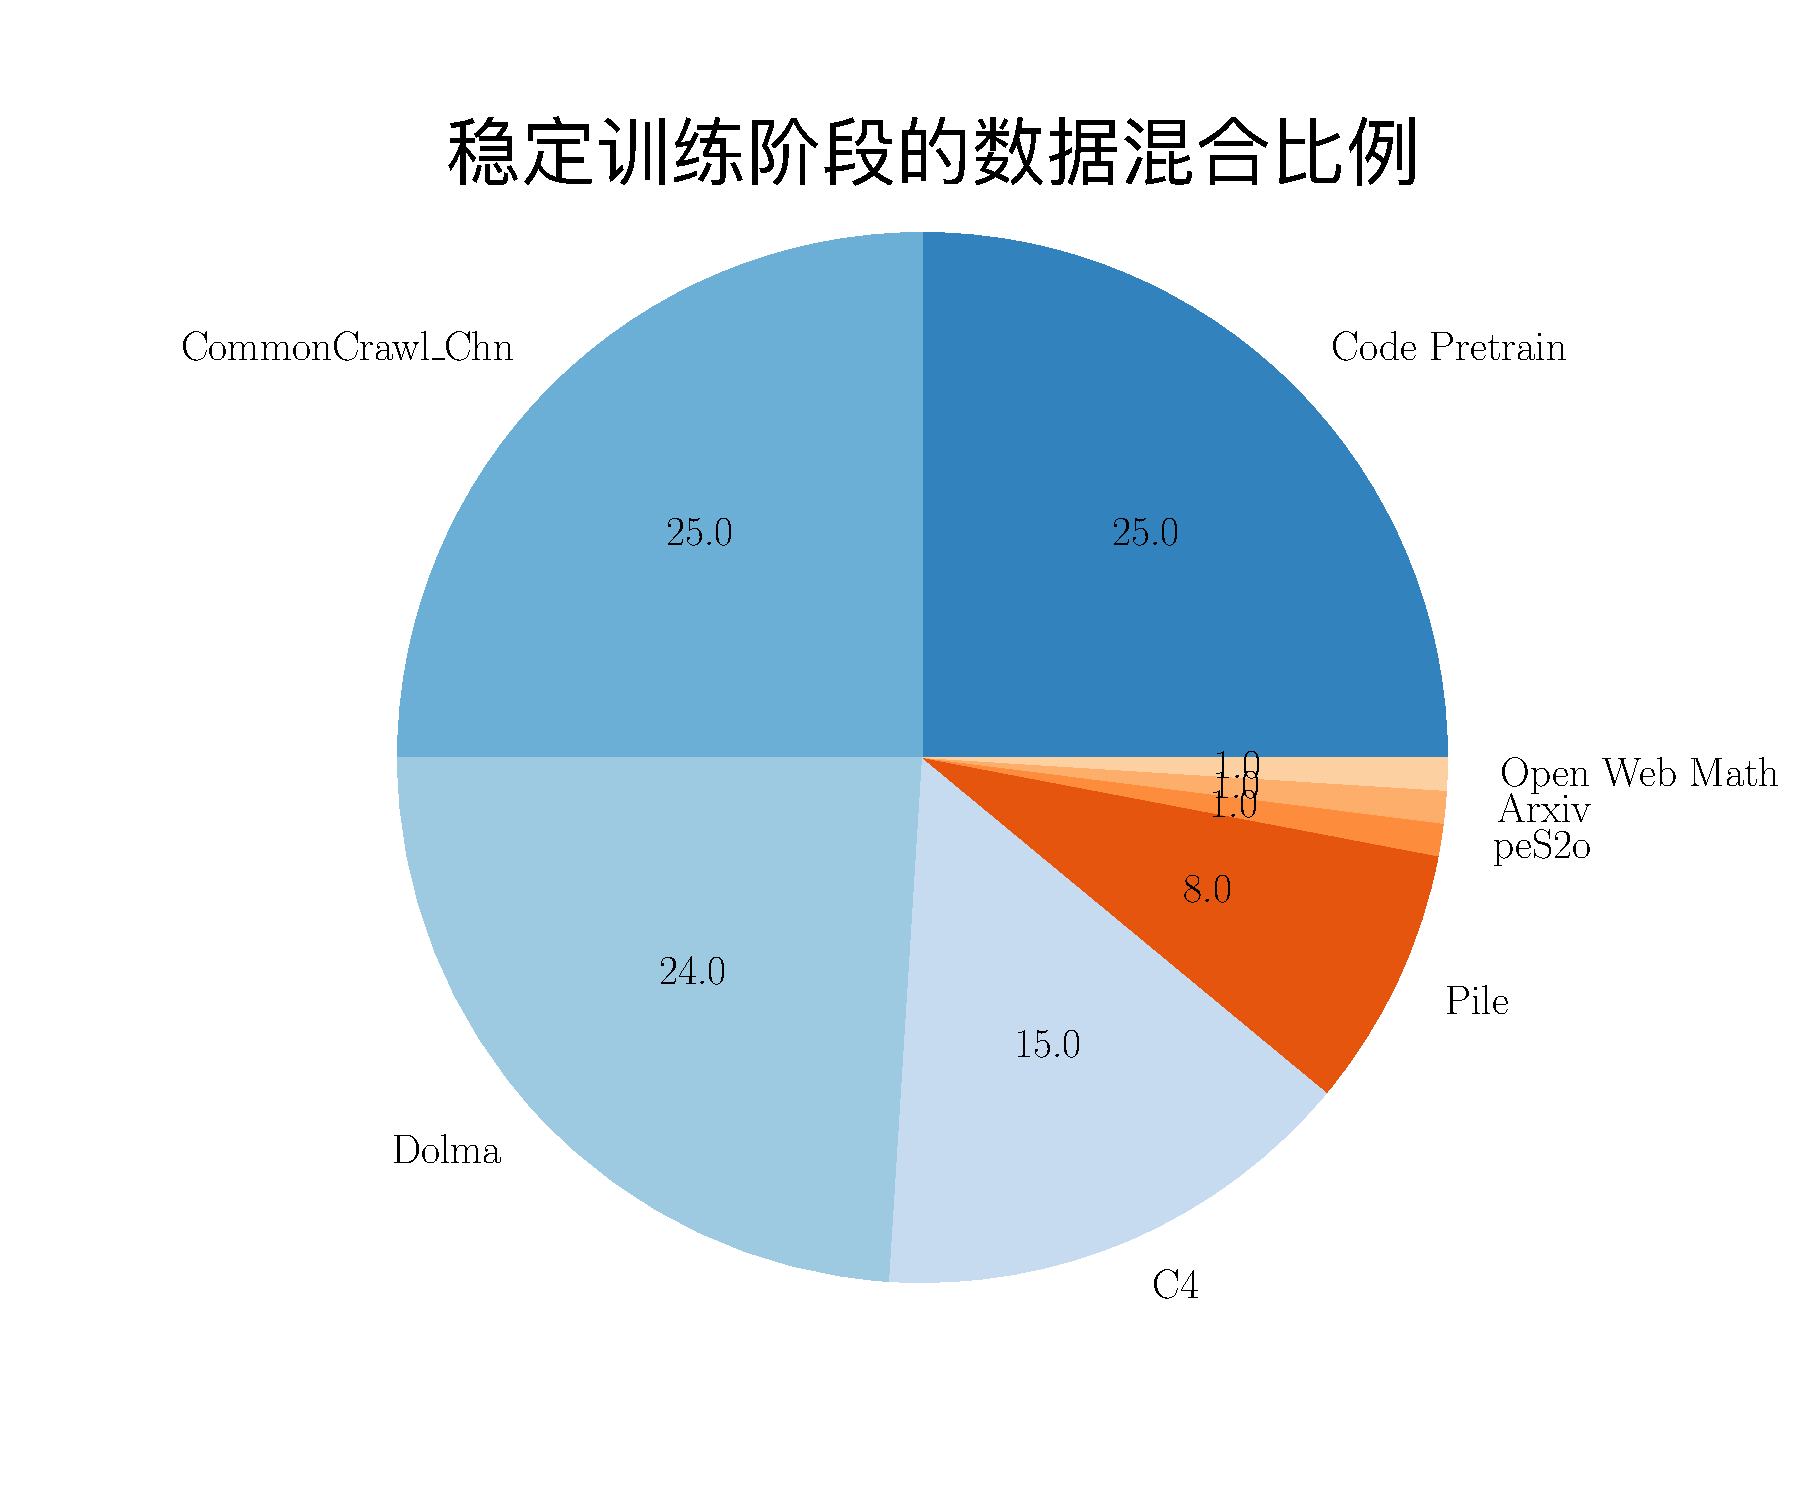
\includegraphics[width=1.0\linewidth]{minicpmFig/stable_mixture.pdf}
    \end{minipage}
    \hfill 
    \begin{minipage}{0.48\linewidth}
        \centering
        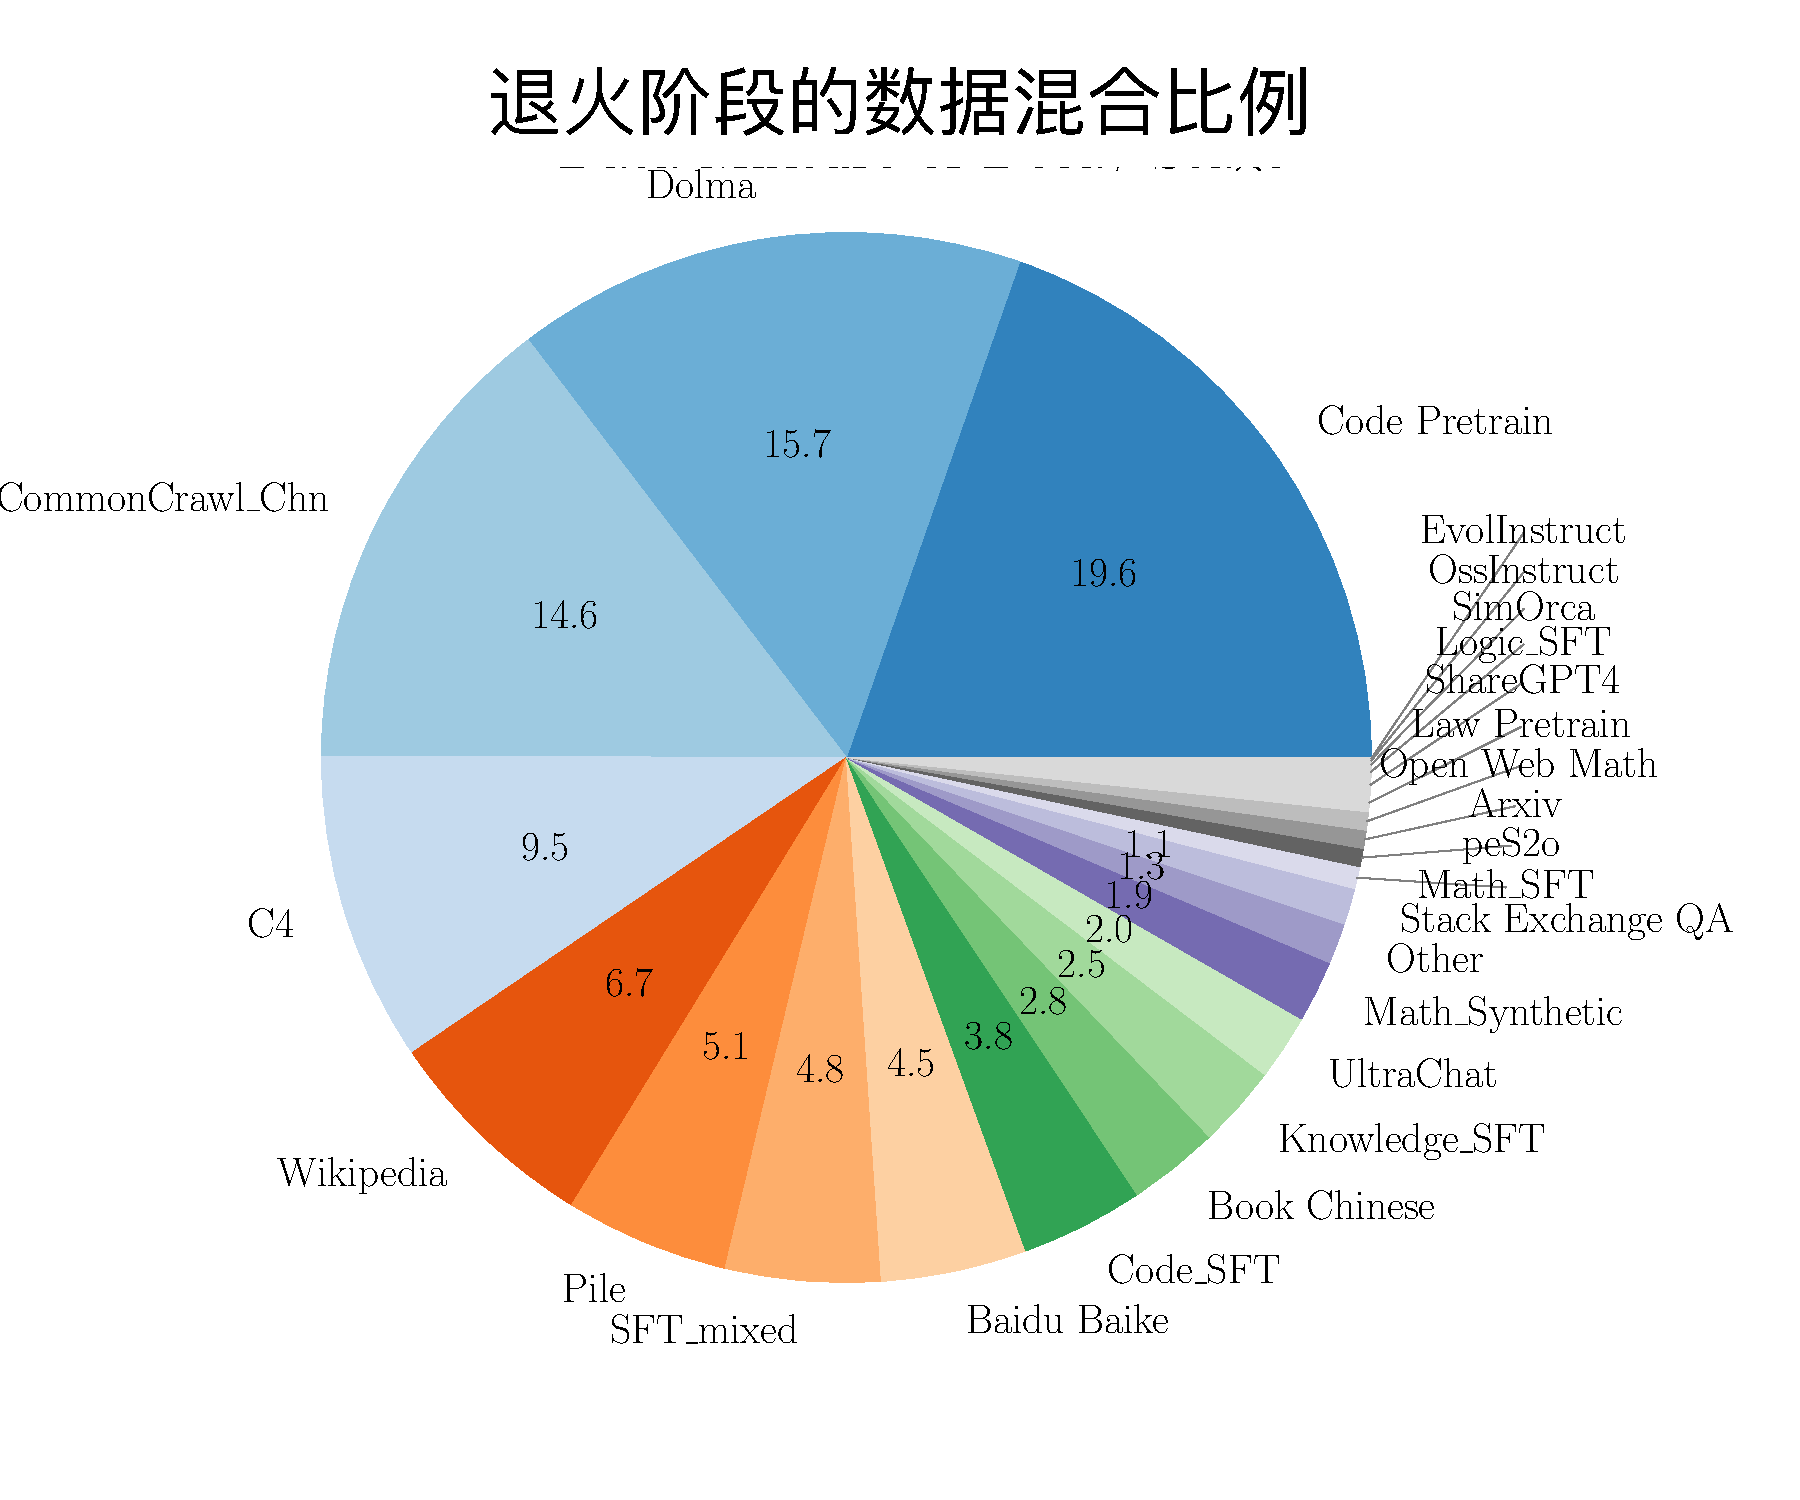
\includegraphics[width=1.0\linewidth]{minicpmFig/decay_data_mixture.pdf}
    \end{minipage}
    \caption{不同训练阶段的数据混合情况。左侧展示的是稳定阶段,右侧展示的是衰减阶段。}
        \label{fig:appdatamixture}
\end{figure}

我们在图\ref{fig:appdatamixture}中介绍训练数据的分布。在图中,CommonCrawl\_Chn是一个中文语料库,源自CommonCrawl原始语料库并经过了全面清理。Dolma~\citep{dolma}、C4~\citep{2019t5}和Pile~\citep{gao2020pile, biderman2022datasheet}是英文语料库。这些语料库内部以及相互之间都使用MinHash算法~\citep{broder1997resemblance}进行了去重。代码预训练数据包含stack~\citep{Kocetkov2022TheStack}和StarCoder~\cite{li2023starcoder},并进行了内部去重和交叉去重。在衰减阶段,混合数据包含更多样化的数据和专有数据,包括UltraChat~\citep{ding2023enhancing}、SlimOrca~\citep{SlimOrca, SlimOrcaDedup}、OssInstruct~\citep{wei2023magicoder}、EvolInstruct~\citep{xu2023wizardlm}。后缀为SFT的数据是我们的专有数据,包括力扣(LeetCode)题目、幼儿园到12年级(K12)的教科书及题目等。 

\subsubsection{训练损失}

\definecolor{darkgreen}{HTML}{476E6B}

在C4数据集上的整体训练损失如图\ref{fig:loss_c4}所示。我们可以看到,正如前期实验所预期的那样,损失在衰减阶段急剧下降。由于我们使用的是指数衰减,在学习率降至最大学习率的10\%以下后,损失仍在下降。然而,因为在衰减阶段之后我们会继续对模型进行监督微调(SFT),所以我们不会使用最终的检查点。我们进行微调所基于的检查点显示在\textcolor{darkgreen}{深绿色}线段的最后一个检查点处。MiniCPM - 1.2B中的首次损失下降是增大批量大小的结果,这可能与降低学习率有类似的效果~\citep{smith2017don}。

\definecolor{orange}{HTML}{FFA500}

\begin{figure}[htbp]
    % 第一个子图的minipage
        \centering
        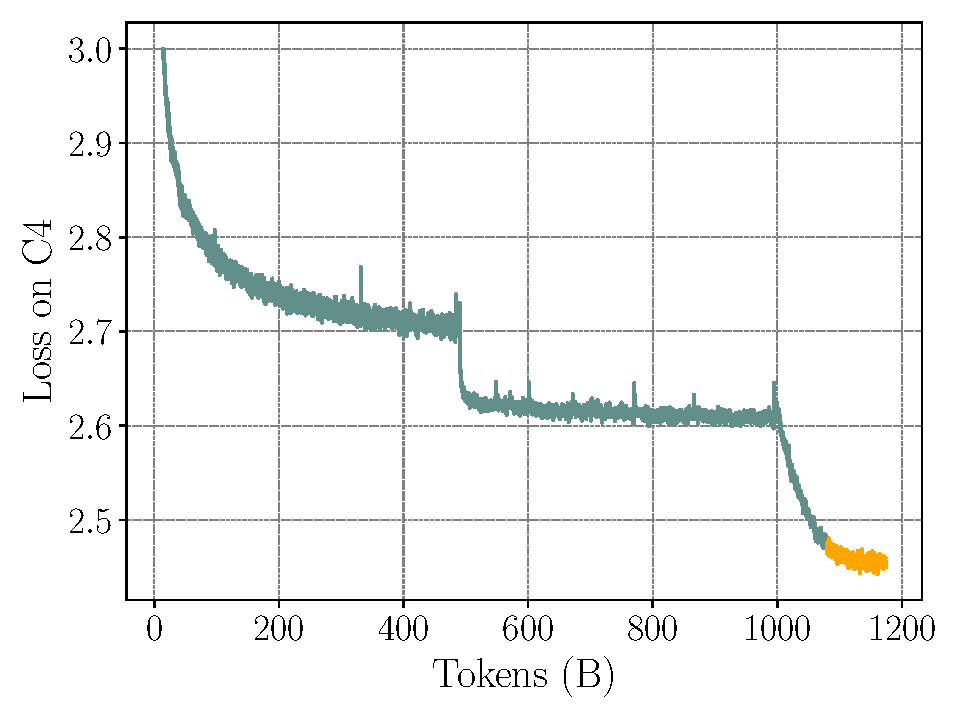
\includegraphics[width=0.9\linewidth]{minicpmFig/1.2B_c4_loss_smoothed.pdf}
    % 第二个子图的minipage
\end{figure}

\begin{figure}[htbp]
    \centering
    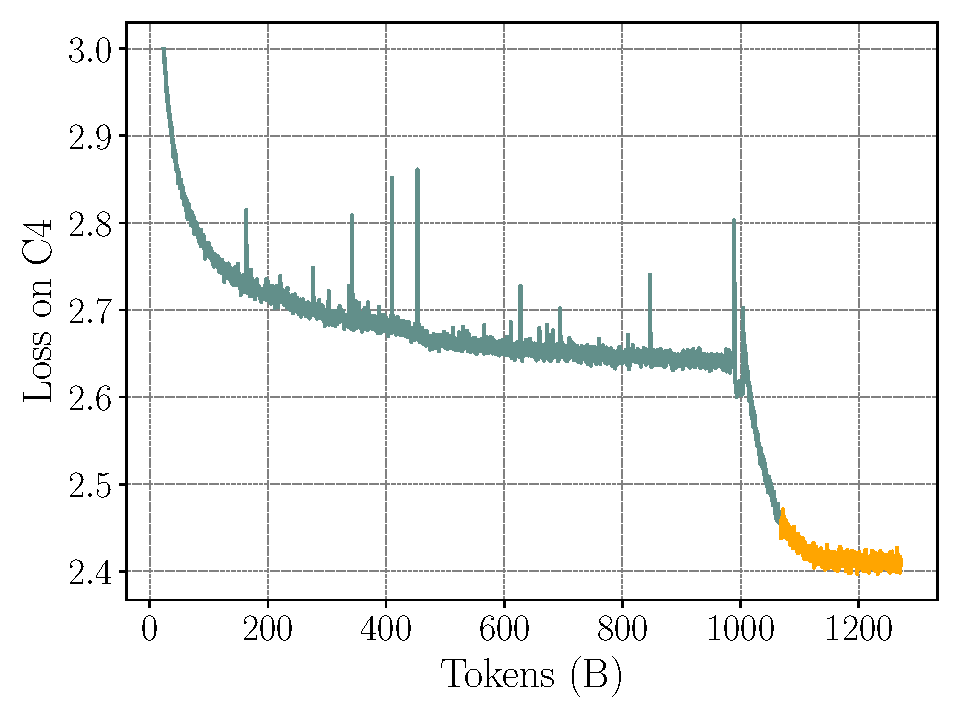
\includegraphics[width=0.9\linewidth]{minicpmFig/2.4B_c4_loss_smoothed.pdf}
    \caption{MiniCPM - 1.2B(左)和MiniCPM - 2.4B(右)在C4数据集上的损失曲线。损失曲线尾部的\textcolor{orange}{橙色}线段表示剩余的衰减过程,MiniCPM发布版本中未使用该部分。}
    \label{fig:loss_c4}
\end{figure}

\section{评估}
\label{sec:evaluation}
整体评估使用我们的开源工具UltraEval\footnote{https://ultraeval.openbmb.cn/home}。UltraEval是一个用于评估基础模型能力的开源框架。它提供了一个轻量级且用户友好的评估系统,支持对主流大模型的性能评估,满足模型训练团队的快速评估需求。其底层推理和加速使用开源框架vLLM~\citep{kwon2023efficient},数据集包括常用数据集:用于评估英语知识的MMLU~\citep{hendrycks2020measuring}、用于评估中文知识的CMMLU~\citep{li2024cmmlu}和C - Eval~\citep{huang2024c}、用于评估编程能力的HumanEval~\citep{chen2021evaluating}和MBPP~\citep{austin2021program}、用于评估数学能力的GSM8K~\citep{cobbe2021training}和MATH~\citep{hendrycks2021measuring}、用于评估常识推理能力的HellaSwag~\citep{zellers2019hellaswag}、ARC - e~\citep{clark2018think}、ARC - c~\citep{clark2018think}以及用于评估逻辑推理能力的BBH~\citep{suzgun2022challenging}。

由于对大模型进行标准化评估存在困难,且许多模型评估缺乏公开可用的提示词和测试代码,我们尽力调整评估方法以适用于各种模型类型。具体而言,在测试时我们从标准化的输入提示词入手,并根据每个模型合适的输入 - 输出模板进行调整。我们仓库中的\textbf{评估脚本和提示词也都是开源的},欢迎开发者不断改进我们的评估方法。

在测试问答任务(ARC - e、ARC - c、HellaSwag)时,通常采用两种方法。第一种是使用困惑度(PPL):我们将每个选项作为问题的延续,并使用选项的困惑度作为选择标准。第二种是直接生成,即模型直接输出答案选项。我们观察到使用这两种方法得到的结果存在显著差异。MiniCPM在直接生成和困惑度测试中的表现相近,在直接生成方面表现更好。另一方面,Mistral - 7B - v0.1在困惑度测试中表现更好,但在直接生成方面表现较差。为解决这一现象,在报告每个模型的分数时,我们采用得分最高的评估方法所得到的分数,以确保比较的公平性。

整体评估结果见表\ref{tab:benchmark}。总体而言,在上述数据集上,我们有以下几点观察。(1) 平均而言,MiniCPM - 2.4B在所有小语言模型(SLMs)中排名最高。(2) MiniCPM - 2.4B在英语方面的表现与Mistral - 7B - v0.1相近,但在中文方面显著优于Mistral - 7B - v0.1。(3) 除了在MMLU、BBH和HellaSwag数据集上,MiniCPM - 2.4B的表现优于Llama2 - 13B;除了在HellaSwag数据集上,MiniCPM - 1.2B的表现优于Llama2 - 7B。(4) 一般来说,与其他知识导向型数据集相比,BBH对小语言模型(SLMs)来说比大语言模型(LLMs)更难,这表明推理能力可能比知识更依赖于模型规模。(5) 在小语言模型(SLMs)中,Phi - 2在学术导向型数据集上的表现与MiniCPM相当。这可能是因为它们的训练数据大多涉及强调教育和学术场景的教科书式数据。由于我们的预训练数据覆盖了更多的数据分布,我们认为MiniCPM在知识和能力覆盖方面表现更好,这在附录\ref{app:cases}中可以看到。 

\section{模型效果}

\begin{table}[!htbp]
    \centering
\scalebox{0.90}{
    \begin{tabular}{lm{1.2cm}m{1.2cm}m{1.2cm}m{1.7cm}m{1.2cm}m{1.2cm}m{1.2cm}m{1.2cm}}
\toprule
\textbf{Model} & \textbf{C-Eval} & \textbf{CMMLU} & \textbf{MMLU} & \textbf{HumanEval} & \textbf{MBPP} & \textbf{GSM8K} & \textbf{MATH}\\
\midrule
Llama2-7B & 32.42 & 31.11 & 44.32 & 12.20 & 27.17 & 13.57 & 1.80\\
Qwen-7B & 58.96 & 60.35 & 57.65 & 17.07 & 42.15 & 41.24 & 5.34\\
Deepseek-7B  & 42.82 & 44.45 & 47.82 & 20.12 & 41.45 & 15.85 & 1.53 \\
Mistral-7B  & 46.12 & 42.96 & 62.69 & 27.44 & 45.20 & 33.13 & 5.00 \\
Gemma-7B  & 42.57 & 44.20 & 60.83 & 38.41 & 50.12 & 47.31 & 6.18\\
\midrule
Llama2-13B  & 37.32 & 37.06 & 54.71 & 17.07 & 32.55 & 21.15 & 2.25\\
MPT-30B  & 29.34 & 32.09 & 46.56 & 21.95 & 35.36 & 10.31 & 1.56 \\
Falcon-40B & 40.29 & 41.57 & 53.53 & 24.39 & 36.53 & 22.44 & 1.92 \\
\midrule
TinyLlama-1.1B & 25.02 & 24.03 & 24.3 & 6.71 & 19.91 & 2.27 & 0.74 \\
Qwen-1.8B & 49.81 & 45.32 & 43.37 & 7.93 & 17.8 & 19.26& 2.42 \\
Qwen1.5-1.8B & \textbf{55.00} & 50.85 & 43.81 & 5.49 & 24.82 & 26.16 & 3.25 \\
Gemini Nano-3B & - & - & - & - & 27.20 & 22.80 & - \\
StableLM-Zephyr-3B & 30.34 & 30.89 & 45.90 & 35.37 & 31.85 & 52.54 & 12.12\\
Phi-2(2B) & 23.37 & 24.18 & 52.66 & 47.56 & \textbf{55.04} & \textbf{57.16} & 3.50 \\
Gemma-2B & 29.26 & 28.56 & 38.49 & 24.39 & 29.74 & 16.83 & 3.34\\
\midrule
\textbf{MiniCPM-1.2B} & 49.14 & 46.81 & 49.63  & 44.51  & 32.75 & 31.77 &  10.60 \\
\textbf{MiniCPM-2.4B} & 51.13 & \textbf{51.07} & \textbf{53.46} & \textbf{50.00 }& 47.31 & 53.83 & \textbf{10.24}\\
\bottomrule
\end{tabular}
}
\scalebox{0.90}{
 \begin{tabular}{lm{1.2cm}m{1.2cm}m{1.2cm}m{1.7cm}m{1.2cm}m{1.2cm}m{1.2cm}m{1.2cm}}
\textbf{Model}  & \textbf{BBH} &\textbf{ARC-e} & \textbf{ARC-c} & \textbf{HellaSwag} & \textbf{Avg} & \textbf{Avg$_{\text{en}}$} & \textbf{Avg$_{\text{chn}}$} \\
\midrule
Llama2-7B  & 33.23 & 75.25$^{\dag}$ & 42.75 & 75.62$^{\dag}$ & 35.40 & 36.21 & 31.77 \\
Qwen-7B  & 37.75 & 83.42 & 64.76 & 75.32$^{\dag}$ & 49.46 & 47.19 & 59.66 \\
Deepseek-7B  & 33.38 & 74.58$^{\dag}$ & 42.15$^{\dag}$ & 75.45$^{\dag}$ & 39.96 & 39.15 & 43.64 \\
Mistral-7B & 41.06 & 83.92 & 70.73 & 80.43$^{\dag}$ & 48.97 & 49.96 & 44.54 \\
Gemma-7B  & 39.19 & 89.35 & 76.79 & 79.47 & 52.22 & 54.18 & 43.39 \\
\midrule
Llama2-13B & 37.92 & 78.87$^{\dag}$ & 58.19 & 79.23$^{\dag}$ & 41.48 & 42.44 & 37.19 \\
MPT-30B  & 38.22 & 78.66$^{\dag}$ & 46.08$^{\dag}$ & 79.72$^{\dag}$ & 38.17 & 39.82 & 30.72 \\
Falcon-40B & 36.24 & 81.94$^{\dag}$ & 57.68 & 83.26$^{\dag}$ & 43.62 & 44.21 & 40.93 \\
\midrule
TinyLlama-1.1B  & 28.78 & 60.77$^{\dag}$ & 28.15$^{\dag}$ & 58.33$^{\dag}$ & 25.36 & 25.55 & 24.53 \\
Qwen-1.8B  & 29.07 & 63.97$^{\dag}$ & 43.69 & 59.28$^{\dag}$ & 34.72 & 31.87 & 47.57 \\
Qwen1.5-1.8B  & 28.82 & 64.86 & 45.56 & 59.39 & 37.09 & 33.57 & \textbf{52.93} \\
Gemini Nano-3B & 42.40 & - & - & - & - & - & - \\
StableLM-Zephyr-3B  & 37.68 & 73.78 & 55.38 & 71.87$^{\dag}$ & 43.46 & 46.32 & 30.62 \\
Phi-2(2B)  & \textbf{43.39} & \textbf{86.11} & \textbf{71.25} & \textbf{73.07$^{\dag}$} & 48.84 & \textbf{54.42} & 23.78 \\
Gemma-2B  & 30.93 & 74.33 & 40.70 & 69.51 & 35.10 & 36.47 & 28.91\\
\midrule
\textbf{MiniCPM-1.2B}  & 34.70 & 80.93 & 66.81 &  \textbf{54.72} &  45.67 & 45.16 & 47.98 \\
\textbf{MiniCPM-2.4B}  & 36.87 & 85.44 & 68.00 & 68.25 & \textbf{52.33} & 52.60 & 51.10 \\
\bottomrule
\end{tabular}
}
\caption{Benchmark Score of MiniCPM-2.4B and MiniCPM-1.2B (both without RLHF). The two tables are continuous horizontally. \textbf{Avg} is over all dataset in the table, \textbf{Avg$_{\text{chn}}$} is the average of C-Eval and CMMLU while \textbf{Avg$_{\text{en}}$} is the average of remaining datasets. $\dag$ means the result is tested using PPL metrics. \textbf{Bold} numbers represent the best score among the SLMs. Results of Gemini Nano-3B are borrowed from ~\cite{team2023gemini}.}
\label{tab:benchmark}
\end{table}
\vspace{-5mm}

\section{MiniCPM - 128K}
涉及长文本上下文的任务依赖于这些上下文中的隐含信息,从而避免了对小语言模型(SLM)通常缺乏的广泛知识的需求。在本节中,我们将MiniCPM - 2.4B的上下文长度从4096个词元扩展到128000个词元,以展示小语言模型有效处理长文本上下文的能力。

\textbf{初始化}:
在初始化时,我们禁用了输入和输出之间的嵌入共享,这主要是为了适应长文本上下文训练所必需的词汇并行性。语言模型(LM)头部从输入嵌入进行初始化。

\textbf{训练}:
与MiniCPM类似,MiniCPM - 2.4B - 128K使用WSD作为其学习率调度器,并复用MiniCPM - 2.4B稳定训练阶段的最后一个检查点。关于训练数据,我们将\ref{sec:appdatadistrbution}节中详细介绍的数据集分布分为“短数据”和“长数据”。我们将书籍、维基百科文章和论文归类为“长数据”,其他数据归类为“短数据”。训练过程中,44%为长数据,56%为短数据,以进行持续训练。对于长文本上下文的扩展,在4K到32K的范围我们应用调整后的基本频率(ABF)~\citep{xiong2023effective},在32K到128K的范围采用NTK感知旋转位置嵌入(RoPE)缩放~\citep{bloc97_2023_ntk}和课程学习。这两个阶段都涉及未来训练。此外,正如易科技报告~\citep{young2024yi}和斑马模型(Zebra)~\citep{song2023zebra}所指出的,我们使用合成的长问答数据,这显著提升了模型在上下文感知任务中的性能。

\textbf{评估}:我们在$\infty$Bench~\citep{zhang2024infty}中对MiniCPM - 2.4B - 128K进行评估,$\infty$Bench是一个用于长文本上下文评估的开创性基准测试。$\infty$Bench~\citep{zhang2024infty}中的任务超越了典型的检索任务,通过长文本上下文推理对模型提出挑战。从表\ref{tab:longcontext}中可以看到,我们取得了与Mistral - 7B - Instruct - v0.2(ABF1000w)相当的结果,并且尽管规模小2.5倍,但性能优于ChatGLM3 - 6B - 128K。 

\section{MiniCPM - MoE(混合专家模型)}
我们进一步利用混合专家(Mixture - of - Expert)方法扩展MiniCPM的能力。

\textbf{初始化}:
MiniCPM - MoE使用稀疏升级(Sparse Upcycling)~\citep{komatsuzaki2022sparse}进行初始化。从MiniCPM稳定阶段得到的密集模型检查点会经历一个转换过程,其中每个多层感知机(MLP)层被一个混合专家(MoE)层替代。这些新的MoE层与密集检查点中的原始MLP层完全相同。路由器参数按照均值为0、方差为0.01的正态分布随机初始化。

\textbf{路由机制}:
MiniCPM - MoE的非嵌入参数总数为136亿。
在训练和推理过程中,每个词元会激活八个专家中的两个,这使得激活参数的数量约为40亿。为防止训练崩溃,在最终训练目标中加入了额外的负载均衡损失(load balancing loss)~\citep{fedus2022switch}。这个辅助损失乘以0.01,该值足够大,以确保分配给不同专家的词元能够均衡分布。

\textbf{训练}:
与MiniCPM类似,我们采用WSD作为学习率调度器。关于训练数据,我们严格遵循\ref{sec:appdatadistrbution}节中指定的分布。在稳定训练和衰减阶段,训练批量大小保持在400万个词元,在监督微调(SFT)阶段减少到200万个词元。预训练阶段(包括持续预训练和衰减阶段)跨越130000步,之后我们注意到提升逐渐减小。基准测试结果详见表\ref{tab:a4_moe_benchmark}。

\begin{table}[htbp]
    \centering
\scalebox{0.80}{
    \begin{tabular}{l|cccccccc}
\toprule
    \textbf{模型} &  \textbf{C - Eval} & \textbf{CMMLU} & \textbf{MMLU} & \textbf{HumanEval} & \textbf{MBPP} & \textbf{GSM8K} & \textbf{MATH} &\textbf{BBH}  \\
\midrule
    Llama2 - 34B & - & - & 62.6 & 22.6 & 33.0$^\dag$ & 42.2 & 6.24 & \textbf{44.1} \\
    Deepseek - MoE(160亿) & 40.6 & 42.5 & 45.0 & 26.8 & 39.2 & 18.8 & 4.3 &  - \\
    Mistral - 7B & 46.12 & 42.96 & \textbf{62.69} & 27.44 & 45.20 & 33.13 & 5.0 & {41.06 }\\
    Gemma - 7B & 42.57 & 44.20 & 60.83 & 38.41 & 50.12 & 47.31 & 6.18 & 39.19 \\
\midrule
    MiniCPM - 2.4B & 51.13 & 51.07 & 53.46 & 50.00 & 47.31 & 53.83 & 10.24 & 36.87 \\
   \textbf{MiniCPM - MoE(136亿)} & \textbf{58.11} & \textbf{58.80} & 58.90 & \textbf{56.71} & \textbf{51.05} & \textbf{61.56} & \textbf{10.52} & 39.22 \\
\bottomrule

    \end{tabular}
}
    \caption{MiniCPM - MoE的基准测试结果。$^\dag$表示MBPP的评估结果基于完整数据集,而非人工验证集~\citep{austin2021program}。Llama2 - 34B和Qwen1.5 - 7B的评估结果取自其技术报告。}
    \label{tab:a4_moe_benchmark}

\end{table}

\section{MiniCPM - DPO(直接偏好优化)}
\label{app:rlhf}
在监督微调(SFT)之后,我们采用直接偏好优化(DPO)~\citep{rafailov2024direct}方法使模型与人类偏好对齐。在此阶段,UltraFeedback~\citep{cui2023ultrafeedback}被用作主要的对齐数据集,同时构建了一个专有偏好数据集,以提升模型在代码和数学方面的能力。由于我们有预定义的训练步数,所以使用余弦退火学习率调度器(Cosine LRS),以$1\times 10^{-5}$的学习率进行一轮DPO训练。

应用DPO进行偏好对齐后,模型在MTBench~\citep{zheng2024judging}上的得分从监督微调后的6.89提升到了7.25,甚至超过了像Llama2 - 70B - Chat这样的大模型(见图\ref{fig:mtbenchscore})。然而,我们也注意到,模型在基准测试中的性能略有下降,这就是所谓的对齐代价(alignment tax)~\citep{askell2021general}。

\begin{table}[htbp]
    \centering
\scalebox{0.87}{

\begin{tabular}{lccccccccc}
\toprule
\textbf{模型} & \textbf{C - Eval} & \textbf{CMMLU} & \textbf{MMLU} & \textbf{HumanEval} & \textbf{MBPP} & \textbf{GSM8K} & \textbf{MATH}\\
\midrule
ChatGLM2 - 6B & 52.05 & 49.21 & 45.77 & 10.37 & 9.38 & 22.74 & 5.96 \\
Mistral - 7B - Instruct - v0.1 & 38.06 & 36.96 & 53.56 & 29.27 & 39.34 & 28.73 & 3.48\\
Mistral - 7B - Instruct - v0.2 & 42.55 & 41.92 & 60.51 & 36.59 & 48.95 & 40.49 & 4.95 \\
Qwen - 7B - Chat & 58.57 & 57.23 & 56.03 & 15.85 & 40.52 & 42.23 & 8.3\\
Yi - 6B - Chat & 70.88 & 71.11 & 62.95 & 14.02 & 28.34 & 36.54 & 3.88\\
Baichuan2 - 7B - Chat & 53.28 & 53.50 & 53.00 & 21.34 & 32.32 & 25.25 & 6.32\\
Deepseek - 7B - chat & 46.95 & 49.72 & 51.67 & 40.85 & 48.48 & 48.52 & 4.26 \\
Llama2 - 7B - Chat & 34.54 & 32.64 & 47.64 & 14.02 & 27.40 & 21.15 & 2.08 \\
\midrule
\textbf{MiniCPM - 2.4B - DPO}  & 48.64 & 48.37 & 53.05 & 51.22 & 48.01 & 53.37 & 9.86\\
\bottomrule
\end{tabular}
}

\scalebox{0.88}{
\begin{tabular}{lccccccc}
\toprule
\textbf{模型}  & \textbf{BBH} &\textbf{ ARC - e} & \textbf{ARC - c} & \textbf{HellaSwag} & \textbf{平均} & \textbf{英文平均} & \textbf{中文平均}  \\
\midrule
ChatGLM2 - 6B  & 32.60 & 74.45 & 56.82 & 58.48$^{\dag}$ & 37.98 & 35.17 & 50.63 \\
Mistral - 7B - Instruct - v0.1  & 39.52 & 81.61 & 63.99 & 73.47$^{\dag}$ & 44.36 & 45.89 & 37.51 \\
Mistral - 7B - Instruct - v0.2  & 39.81 & 86.28 & 73.38 & 84.55$^{\dag}$ & 50.91 & 52.83 & 42.24 \\
Qwen - 7B - Chat  & 37.34 & 64.44$^{\dag}$ & 39.25$^{\dag}$ & 74.52$^{\dag}$ & 44.93 & 42.05 & 57.90 \\
Yi - 6B - Chat  & 37.43 & 84.89 & 70.39 & 74.60$^{\dag}$ & 50.46 & 45.89 & 71.00 \\
Baichuan2 - 7B - Chat  & 37.46 & 79.63 & 60.15 & 69.23$^{\dag}$ & 44.68 & 42.74 & 53.39 \\
Deepseek - 7B - chat  & 35.70 & 76.85 & 63.05 & 76.68$^{\dag}$ & 49.34 & 49.56 & 48.34 \\
Llama2 - 7B - Chat  & 35.54 & 74.28 & 54.78 & 75.65$^{\dag}$ & 38.16 & 39.17 & 33.59 \\
\midrule
\textbf{MiniCPM - 2.4B - DPO}  & 36.22 & 85.02 & 68.17 & 65.67 & 51.60 & 52.29 & 48.51 \\
\bottomrule
\end{tabular}
}
\caption{MiniCPM - 2.4B - DPO与更大的聊天模型的基准测试得分对比。}
\label{tab:benchmark}
\end{table}


\begin{figure}
    \centering
    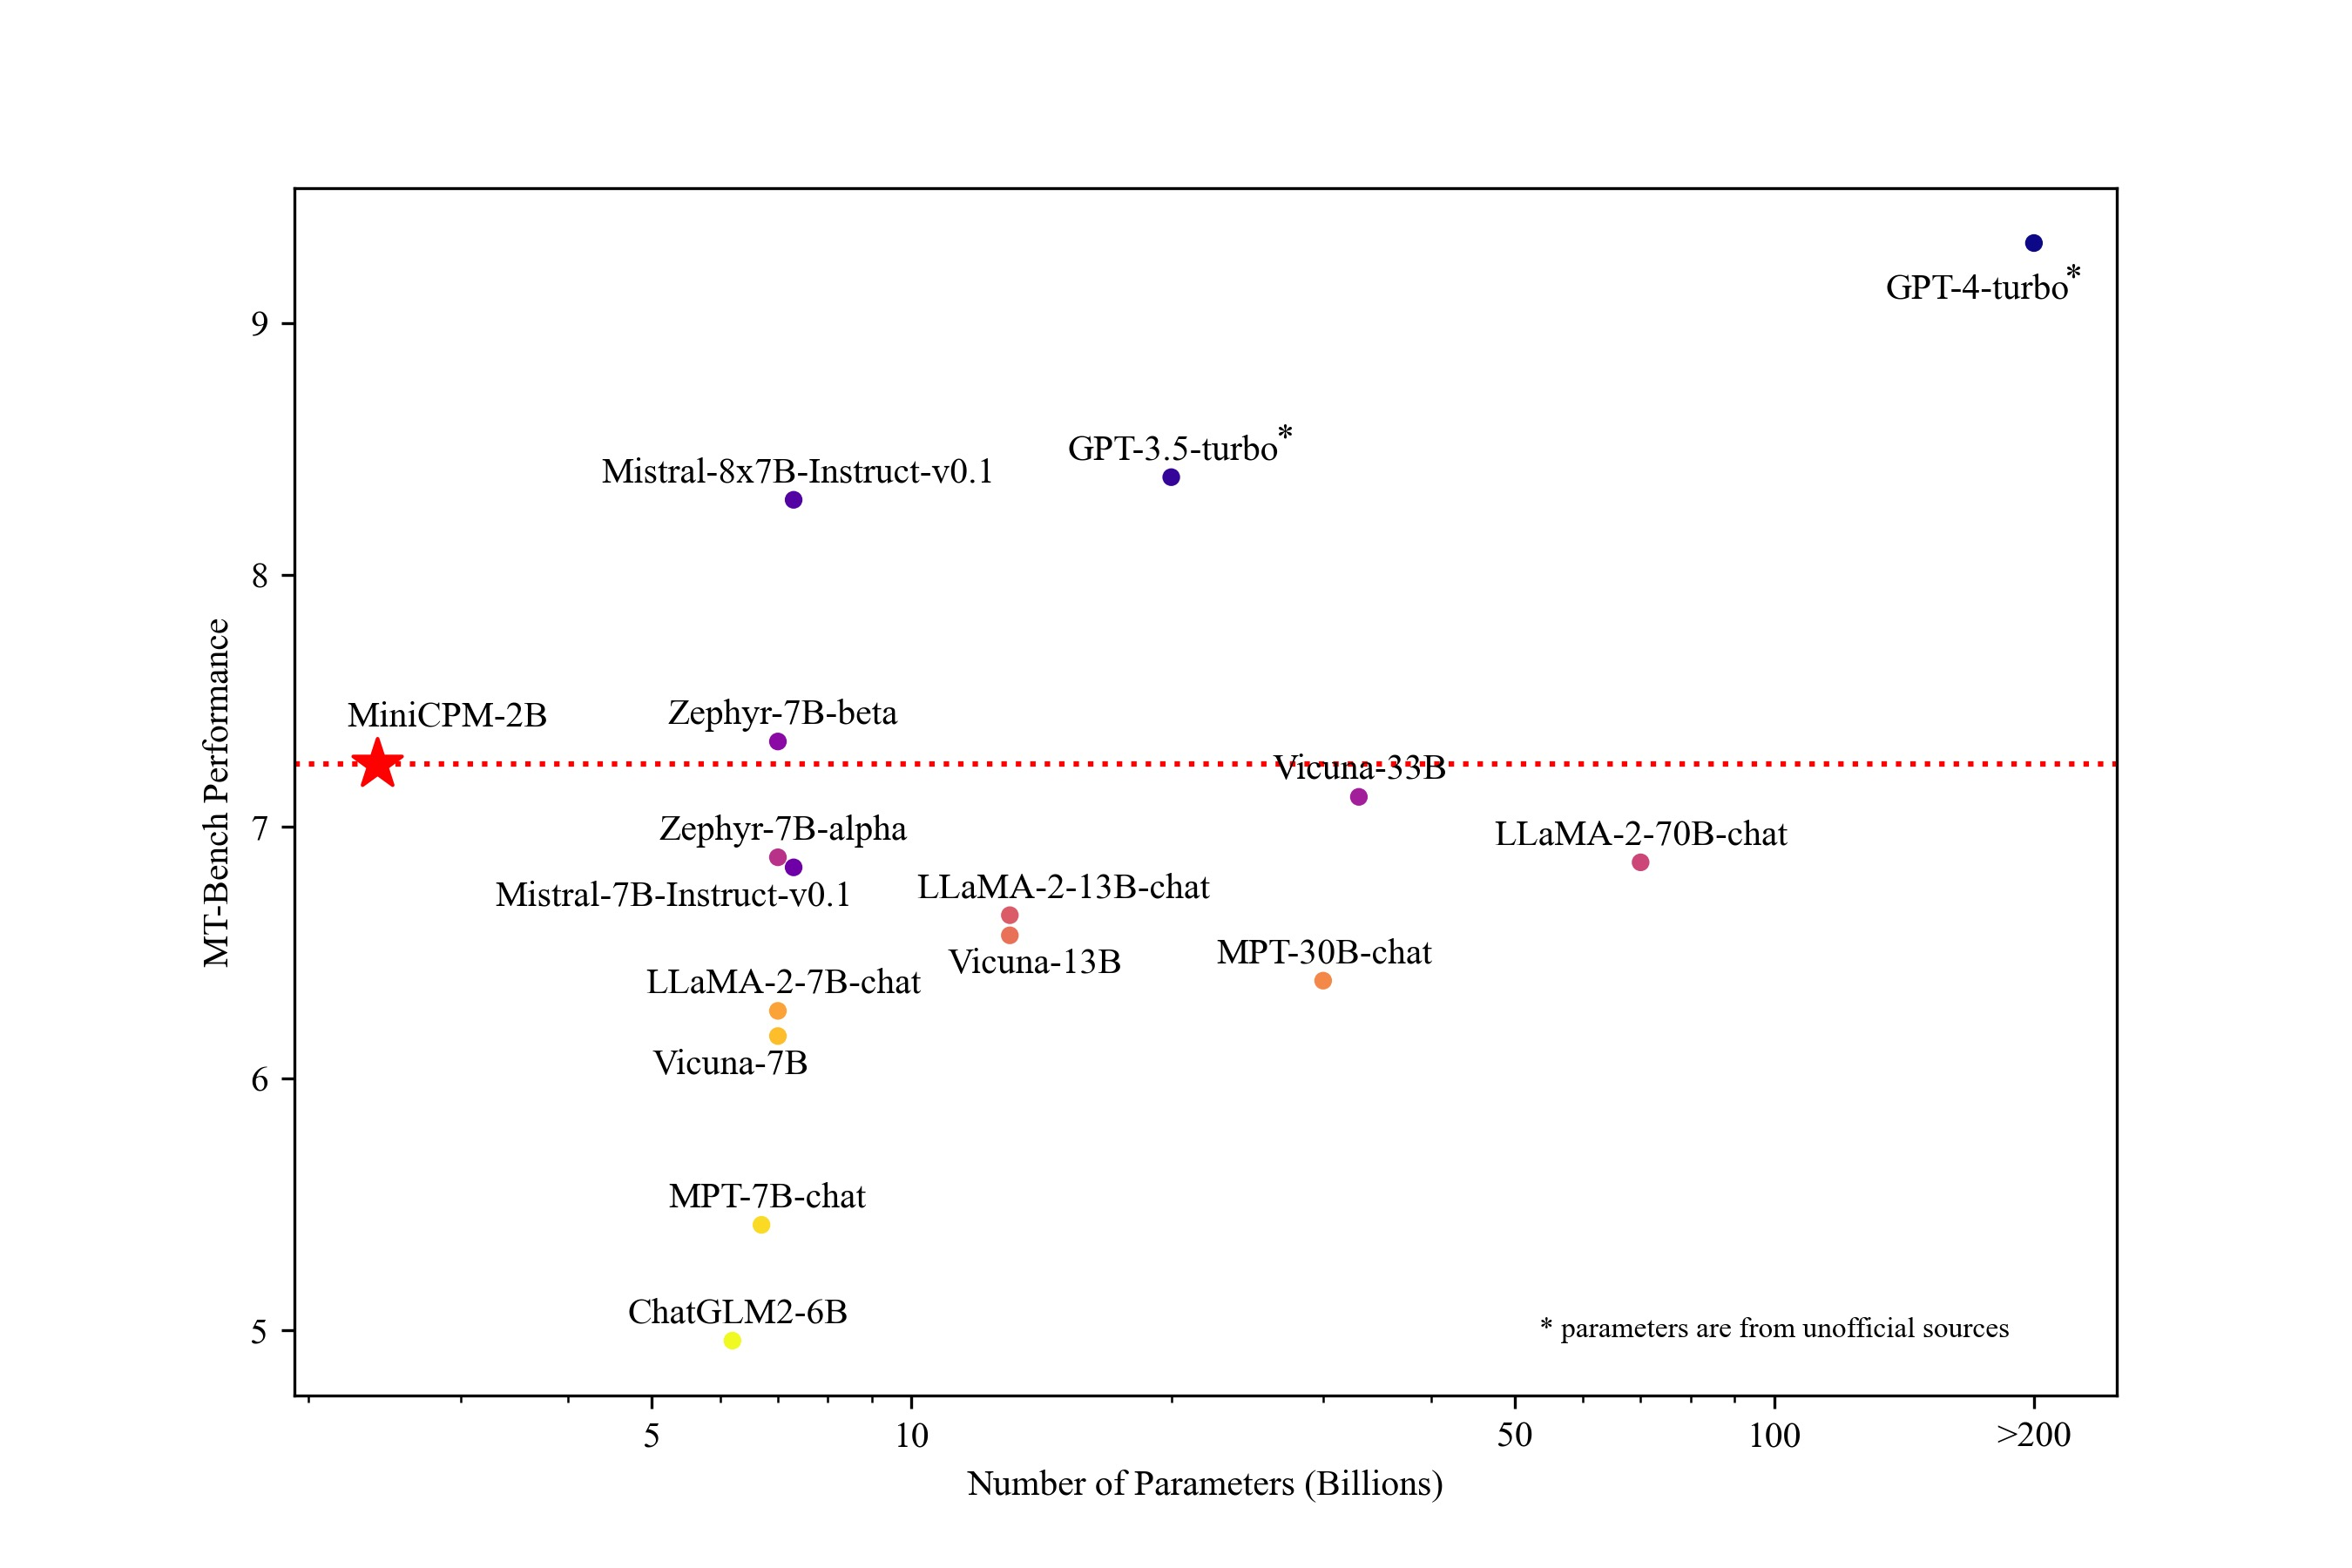
\includegraphics[width=\linewidth]{minicpmFig/mtbench_graph.jpg}
    \caption{MiniCPM - DPO - 2.4B的MTBench得分超过了许多更大规模的模型。}
    \label{fig:mtbenchscore}
\end{figure}

\section{模型能力展示}
MiniCPM系列与微软的Phi~\citep{li2023textbooks}等其他强大的小语言模型(SLMs)相比,一个显著区别在于,我们使用通用语料库来训练MiniCPM,这确保了模型在各种任务中的通用性和泛化能力。在本节中,我们展示几个通常只有更大规模模型才能实现的有趣生成实例,以展现MiniCPM的能力。尽管我们并未对训练集中是否存在特定案例进行广泛排查,但考虑到这些案例的表达方式多样,我们确保没有刻意添加与测试案例相似的数据。 

\begin{figure}[!h]
    \centering
    \scalebox{0.95}{
    \begin{AIbox}{Translation}
    {\bf Prompt:} 
    {\scriptsize
    Translate this sentence into French: "I am a freshman on Chinese, do you know how this sentence is translated: {如何用Python创建一个简单的网页爬虫?" (\textcolor{darkgreen}{How to create a simple web crawler in Python?})
    }}\\\ \\
    \parbox[t]{0.49\linewidth}{{\bf MiniCPM-1.2B:}\\
    \scriptsize
    Je suis un homme nouveau en chinois, vous êtes-vous au courant de la manière dont cette phrase est traduite : Comment créer un petit scraper web simple à Python ?
    }\hspace{0.02\linewidth}%
    \parbox[t]{0.49\linewidth}{{\bf MiniCPM-2.4B-DPO:} \\
    \scriptsize
    Je suis un nouveau-né en chinois, sais-tu comment on crée un simple web crawler en Python ?
    Translation: "Je suis un nouveau-né en chinois, sais-tu comment on crée un simple web crawler en Python ?"
    }
    \hspace{0.01\linewidth}
    \end{AIbox}
    }
    \caption{Examples on translation. We notice that MiniCPM-2.4B-DPO performs better in translating the technical part, but both models are unnatural in expressing "just starting to learn Chinese.". However, both models successfully understand the instruction with traps and generate French despite we do not include French corpus intentionally.}
    \label{fig:translation_example}
\end{figure}
    
    
\begin{figure}[!h]
    \centering
    \scalebox{0.95}{
    \begin{AIbox}{Math and Reasoning}
    {\bf Prompt:} 
    {\scriptsize
    {如果以下算式中减号均表示加号,而加号实际上是减号,给出算式的计算结果15-25-12+34=
    }\\ (\textcolor{darkgreen}{If in the following equation, minus signs represent addition, and plus signs represent subtraction, give the result of the calculation: 15-25-12+34=})}\\\ \\
    \parbox[t]{0.49\linewidth}{{\bf MiniCPM-1.2B:}\\
    \scriptsize
    {如果减号表示加号,那么我们可以将算式改写为:15 + 25 + 12 - 34 \\ \\
    首先计算前两个数的和:15 + 25 = 40\\
    然后计算前三个数的和:40 + 12 = 52\\
    最后计算最后一个数减去前三个数的和:52 - 34 = 18\\ \\
    所以,算式的计算结果为18。}\\(\textcolor{darkgreen}{If the minus sign represents a plus sign, then we can rewrite the equation as: 15 + 25 + 12 - 34.\\ \\
    First, calculate the sum of the first two numbers: 15 + 25 = 40. \\
    Then, calculate the sum of the first three numbers: 40 + 12 = 52. \\
    Finally, calculate the difference between the last number and the sum of the first three numbers: 52 - 34 = 18. \\ \\
    Therefore, the result of the equation is 18.})
    }
    \hspace{0.02\linewidth}%
    \parbox[t]{0.49\linewidth}{{\bf MiniCPM-2.4B-DPO:} \\
    \scriptsize
    {如果减号均表示加号,而加号实际上是减号,那么算式可以重新表示为:\\
    15+25+12-34\\ \\
    现在我们可以按照加减法的顺序进行计算:\\
    (15+25)+12-34=40+12-34=52-34=18\\ \\
    所以,最终的计算结果是 18。}\\(\textcolor{darkgreen}{If minus signs all represent addition, and plus signs actually represent subtraction, then the equation can be re-expressed as:\\
    15+25+12-34.\\ \\
    Now we can calculate according to the order of addition and subtraction:\\
    (15+25)+12-34 = 40+12-34 = 52-34 = 18\\ \\
    So, the final result of the calculation is 18.})
    }
    \hspace{0.01\linewidth}
    \end{AIbox}
    }
    \caption{Examples on math and reasoning. Both models are successful in symbolic substitution and math calculation.}
    \label{fig:math}
    \end{figure}
    
    \begin{figure}[!b]
    \centering
    \scalebox{0.95}{
    \begin{AIbox}{Instruction Following}
    {\bf Prompt:} 
    {\scriptsize
    {写藏头诗,藏头是龙年大吉
    }\\ (\textcolor{darkgreen}{Writing an acrostic poem, with the hidden message "Good luck in the Year of the Dragon."})}\\\ \\
    \parbox[t]{0.49\linewidth}{{\bf MiniCPM-1.2B:}\\
    \scriptsize
    {龙池春水涨,\\凤阙日初长。\\吉庆何时至,\\太平有象藏。}\\(\textcolor{darkgreen}{The spring water in the dragon's pool rises,\\
    The sun rises at the phoenix gate.\\
    When will good fortune arrive,\\
    Peace and prosperity are hidden in signs.})
    }
    \hspace{0.02\linewidth}%
    \parbox[t]{0.49\linewidth}{{\bf MiniCPM-2.4B-DPO:} \\
    \scriptsize
    {龙腾万里气如虹,\\
    年岁新来乐事浓。\\
    大吉良辰堪共赏,\\
    吉祥如意笑颜红。} \\(\textcolor{darkgreen}{Dragons soar for thousands of miles, their energy like a rainbow,\\
    As the new year begins, joyous occasions abound.\\
    Auspicious days are worth enjoying together,\\
    Good fortune and happiness bring rosy smiles.})
    }
    \hspace{0.01\linewidth}
    \end{AIbox}
    }
    \caption{Examples on instruction following. MiniCPM-2.4B-DPO successfully follows the instructions and generates a poem with the correct tonal pattern and the first character of each sentence. However, MiniCPM-1.2B only generates the correct tonal pattern.}
    \label{fig:instruction}
    \end{figure}
    
    
    
    \begin{figure}[]
    \centering
    \scalebox{0.95}{
    \begin{AIbox}{Emoji}
    {\bf Prompt:} 
    {\scriptsize
    {请给我一个json,每个key是一个emoji, 每个value是这个emoji对应的意思,给出10个左右
    }\\ (\textcolor{darkgreen}{Please give me a JSON object where each key is an emoji and each value is the meaning of that emoji, providing around 10 examples.})}\\\ \\
    \parbox[t]{0.49\linewidth}{{\bf MiniCPM-1.2B:}\\
    \scriptsize
    {当然可以,这是一个包含10个左右emoji及其含义的JSON:\\
    \{\\
    "
\includegraphics[height=10pt]{minicpmFig/smiling-face-with-smiling-eyes_1f60a.png}": "笑容", \\
    "
\includegraphics[height=10pt]{minicpmFig/face-with-tears-of-joy_1f602.png}": "笑", \\
    "
\includegraphics[height=10pt]{minicpmFig/smiling-face-with-heart-eyes_1f60d.png}": "惊叹", \\
    "
\includegraphics[height=10pt]{minicpmFig/face-blowing-a-kiss_1f618.png}": "亲吻", \\
    "
\includegraphics[height=10pt]{minicpmFig/winking-face-with-tongue_1f61c.png}": "恶作剧",\\
    "
\includegraphics[height=10pt]{minicpmFig/pensive-face_1f614.png}": "失望", \\
    "
\includegraphics[height=10pt]{minicpmFig/thinking-face_1f914.png}":"思考", \\
    "
\includegraphics[height=10pt]{minicpmFig/money-mouth-face_1f911.png}": "金钱",\\
    "
\includegraphics[height=10pt]{minicpmFig/folded-hands_1f64f.png}": "帮助",\\
    "
\includegraphics[height=10pt]{minicpmFig/pile-of-poo_1f4a9.png}": "废物"\\
    \} \\
    希望这个JSON对你有帮助!} \\ (\textcolor{darkgreen}{Of course, this is a JSON file containing around 10 emojis and their meanings:\\
    \{\\
    "
\includegraphics[height=10pt]{minicpmFig/smiling-face-with-smiling-eyes_1f60a.png}": "smiling", \\
    "
\includegraphics[height=10pt]{minicpmFig/face-with-tears-of-joy_1f602.png}": "laughing", \\
    "
\includegraphics[height=10pt]{minicpmFig/smiling-face-with-heart-eyes_1f60d.png}": "amazing", \\
    "
\includegraphics[height=10pt]{minicpmFig/face-blowing-a-kiss_1f618.png}": "kissing", \\
    "
\includegraphics[height=10pt]{minicpmFig/winking-face-with-tongue_1f61c.png}": "mischief",\\
    "
\includegraphics[height=10pt]{minicpmFig/pensive-face_1f614.png}": "disappointment", \\
    "
\includegraphics[height=10pt]{minicpmFig/thinking-face_1f914.png}":"thinking", \\
    "
\includegraphics[height=10pt]{minicpmFig/money-mouth-face_1f911.png}": "money",\\
    "
\includegraphics[height=10pt]{minicpmFig/folded-hands_1f64f.png}": "help",\\
    "
\includegraphics[height=10pt]{minicpmFig/pile-of-poo_1f4a9.png}": "rubbish"\\
    \} \\
    Hope you found this JSON useful!})
    }
    \hspace{0.02\linewidth}%
    \parbox[t]{0.49\linewidth}{{\bf MiniCPM-2.4B-DPO:} \\
    \scriptsize
    {当然可以!以下是一个包含10个emoi及其对应意义的JSON对象:\\
    \{\\
    "
\includegraphics[height=10pt]{minicpmFig/smiling-face-with-smiling-eyes_1f60a.png}": "表示愉快或满意,通常用于表达微笑和喜悦。", \\
    "
\includegraphics[height=10pt]{minicpmFig/pouting-face_1f621.png}": "表示愤怒或不满,通常用于表达情绪的激动。", \\
    "
\includegraphics[height=10pt]{minicpmFig/face-with-tears-of-joy_1f602.png}": "表示大笑或开心,通常用于表达笑声和欢乐。", \\
    "
\includegraphics[height=10pt]{minicpmFig/rolling-on-the-floor-laughing_1f923.png}": "表示搞笑或尴尬,通常用于表达搞笑的场景或尴尬的情况。", \\
    "
\includegraphics[height=10pt]{minicpmFig/exploding-head_1f92f.png}": "表示惊讶或震惊,通常用于表达对某个事件或情況的强烈反应。",\\
    "
\includegraphics[height=10pt]{minicpmFig/pensive-face_1f614.png}": "表示失望或沮丧,通常用于表达对某事或某人失去兴趣或信心的情绪。", \\
    "
\includegraphics[height=10pt]{minicpmFig/broken-heart_1f494.png}":"表示心痛或伤心,通常用于表达对某事或某人造成痛苦的强烈感受。", \\
    "
\includegraphics[height=10pt]{minicpmFig/light-bulb_1f4a1.png}": "表示惊喜或兴奋,通常用于表达对某事或某人的发现或发现的情绪。",\\
    "
\includegraphics[height=10pt]{minicpmFig/smiling-face-with-smiling-eyes_1f60a.png}": "表示酷或时髦,通常用于表达自信、独立和潮流的态度。",\\
    "
\includegraphics[height=10pt]{minicpmFig/smiling-face-with-heart-eyes_1f60d.png}": "表示喜欢或欣赏,通常用于表达对某物或某人的喜爱之情。"\\
    \} \\
    希望这个JSON对象能满足您的需求!如果您有任何问题,请随时告诉我。} \\(\textcolor{darkgreen}{Of course! Here is a JSON object containing 10 emojis and their corresponding meanings:\\
    \{\\
    "
\includegraphics[height=10pt]{minicpmFig/smiling-face-with-smiling-eyes_1f60a.png}": "It means happy or satisfied, typically used to express smiling and joy.", \\
    "
\includegraphics[height=10pt]{minicpmFig/pouting-face_1f621.png}": "It means anger or dissatisfaction, typically used to express intense emotions.", \\
    "
\includegraphics[height=10pt]{minicpmFig/face-with-tears-of-joy_1f602.png}": "It means laughing or happy, typically used to express laughter and joy.", \\
    "
\includegraphics[height=10pt]{minicpmFig/rolling-on-the-floor-laughing_1f923.png}": "It means funny or awkward, typically used to express humorous situations or awkwardness.", \\
    "
\includegraphics[height=10pt]{minicpmFig/exploding-head_1f92f.png}": "It means surprise or shock, typically used to express a strong reaction to an event or situation.",\\
    "
\includegraphics[height=10pt]{minicpmFig/pensive-face_1f614.png}": "It means disappointment or discouragement, typically used to express a loss of interest or confidence in something or someone.", \\
    "
\includegraphics[height=10pt]{minicpmFig/broken-heart_1f494.png}": "It means heartache or sadness, typically used to express intense feelings of pain caused by something or someone.", \\
    "
\includegraphics[height=10pt]{minicpmFig/light-bulb_1f4a1.png}": "It means surprise or excitement, typically used to express the emotion of discovery or finding something or someone.",\\
    "
\includegraphics[height=10pt]{minicpmFig/smiling-face-with-smiling-eyes_1f60a.png}": "It means cool or stylish, typically used to express a confident, independent, and trendy attitude.",\\
    "
\includegraphics[height=10pt]{minicpmFig/smiling-face-with-heart-eyes_1f60d.png}": "It means like or appreciate, typically used to express affection or admiration for something or someone."\\
    \} \\
    I hope this JSON object meets your needs! If you have any questions, please feel free to let me know.})
    }
    \hspace{0.01\linewidth}
    \end{AIbox}
    }
    \caption{Examples on emoji. Both models understand emojis and structured data well, and accurately control the number of items implicitly. The DPO model tends to generate more words. }
    \label{fig:emoji}
    \end{figure}